\documentclass[a4paper, 12pt]{article}
\usepackage[utf8]{inputenc}

\usepackage[a4paper,top=1.3cm,bottom=2cm,left=1.5cm,right=1.5cm,marginparwidth=0.75cm]{geometry}
\usepackage{cmap}				
\usepackage{mathtext} 				
\usepackage[T2A]{fontenc}			
\usepackage[utf8]{inputenc}			
\usepackage[english,russian]{babel}	
\usepackage{multirow}
\usepackage{mathtools}
\mathtoolsset{showonlyrefs=true}

\usepackage{graphicx}
\usepackage{wrapfig}
\usepackage{tabularx}
\usepackage{caption}

\title{2.1.3-theory}
\author{Влад Черниенко}
\date{March 2022}


\begin{document}

    \begin{titlepage}
    
        \begin{center}
            {\large МОСКОВСКИЙ ФИЗИКО-ТЕХНИЧЕСКИЙ ИНСТИТУТ (НАЦИОНАЛЬНЫЙ ИССЛЕДОВАТЕЛЬСКИЙ УНИВЕРСИТЕТ)}
        \end{center}
        \begin{center}
            {\large Физтех-школа радиотехники и компьютерных технологий}
        \end{center}
        
        \vspace{4.5cm}
        
        {\huge
            \begin{center}
                {\bf Лабораторная работа 3.2.1} \\
                Сдвиг фаз в цепи переменного тока
            \end{center}
        }
        
        \vspace{12cm}
        
        \begin{flushright}
            {\LARGE Автор: \\ Черниенко Владислав Антонович \\ \vspace{0.2cm} Группа Б01-110}
        \end{flushright}
        
    \end{titlepage}
    
    
    \noindent {\bf Цель работы:} изучить влияние активного сопротивления, индуктивности и ёмкости на сдвиг фаз между током и напряжением в цепи переменного тока.\\
    
    \noindent {\bf В работе используются:} генератор звуковой частоты (ЗГ), двухканальный осциллограф (ЭО), магазин ёмкостей, магазин сопротивлений, катушка индуктивности, резисторы, универсальный измеритель импеданса ($LCR$-метр).\\
    
    \begin{flushleft}
        {\Large {\bf Теоретические сведения}}
    \end{flushleft}
    
    Удобным, хотя и не очень точным, прибором для измерения фазовых соотношений служит электронный осциллограф. Можно предложить два способа измерения разности фаз.
    
    В первом способе два сигнала $U_1$ и $U_2$ подаются на горизонтальную (канал $X$) и вертикальную (канал $Y$) развёртки осциллографа. Смещение луча по горизонтали и вертикали определяется выражениями
    \begin{equation}
        x = x_0 \cdot \mathrm{cos}(\omega t), \hspace{1cm} y = y_0 \cdot \mathrm{cos}(\omega t + \psi),
    \end{equation}
    где $\psi$ — сдвиг фаз между напряжениями $U_1$ и $U_2$, а $x_0$ и $y_0$ — амплитуды напряжений, умноженные на коэффициенты усиления соответствующих каналов осциллографа. Исключив время, после несложных преобразований найдём
    \begin{equation}
        \left( \frac{x}{x_0} \right)^2 + \left( \frac{y}{y_0} \right)^2 + \frac{2 x y}{x_0 y_0} \mathrm{cos}\psi = \mathrm{sin}^2\psi.
    \end{equation}
    
    Полученное выражение определяет эллипс, описываемый электронным лучом на экране осциллографа. Ориентация эллипса зависит как от искомого угла $\psi$, так и от усиления каналов осциллографа. Для расчёта сдвига фаз можно измерить отрезки $2y_{x=0}$ и $2y_0$ (или $2x_{y=0}$ и $2x_0$) и, подставляя эти значения в уравнение эллипса, найти
    \begin{equation}
        \psi = \pm \mathrm{arcsin} \left( \frac{y_{x=0}}{y_0} \right).
        \label{eq1}
    \end{equation}
    Для правильного измерения отрезка $2y_{x=0}$ важно, \textit{чтобы центр эллипса лежал на оси $y$}.
    
    Второй способ заключается в непосредственном измерении сдвига фаз между сигналами на экране двухканального осциллографа. Напряжения $U_1$ и $U_2$ одновременно подаются на входные каналы ЭО при включённой внутренней горизонтальной развёртке. При этом сигналы одновременно отображаются на экране. Измерение разности фаз в таком случае удобно проводить следующим образом:
    \begin{enumerate}
        \item[1)] подобрать частоту горизонтальной развёртки, при которой на экране укладывается чуть больше половины периода синусоиды;
        \item[2)] отцентрировать горизонтальную ось;
        \item[3)] измерить расстояние $x_0$ (см. рис. \ref{pic1}) между нулевыми значениями \textit{одного} из сигналов, что соответствует разности фаз $\pi$;
        \item[4)] измерить расстояние $x$ между нулевыми значениями двух синусоид и пересчитать в сдвиг по фазе: $\psi = \pi x / x_0$. На рис. \ref{pic1} синусоиды на экране ЭО сдвинуты по фазе на $\pi / 2$.
    \end{enumerate}
    
    \newpage
    
    \begin{flushleft}
        {\Large {\bf Экспериментальная установка}}
    \end{flushleft}
    
    Схема установки для исследования сдвига фаз между током и напряжением в цепи переменного тока представлена на рис. \ref{pic1}. Эталонная катушка $L$, магазин ёмкостей $C$ и магазин сопротивлений $R$ соединены последовательно и через дополнительное сопротивление $r$ подключены к источнику синусоидального напряжения — звуковому генератору (ЗГ).
    
    \begin{figure}[ht]
        \centering
        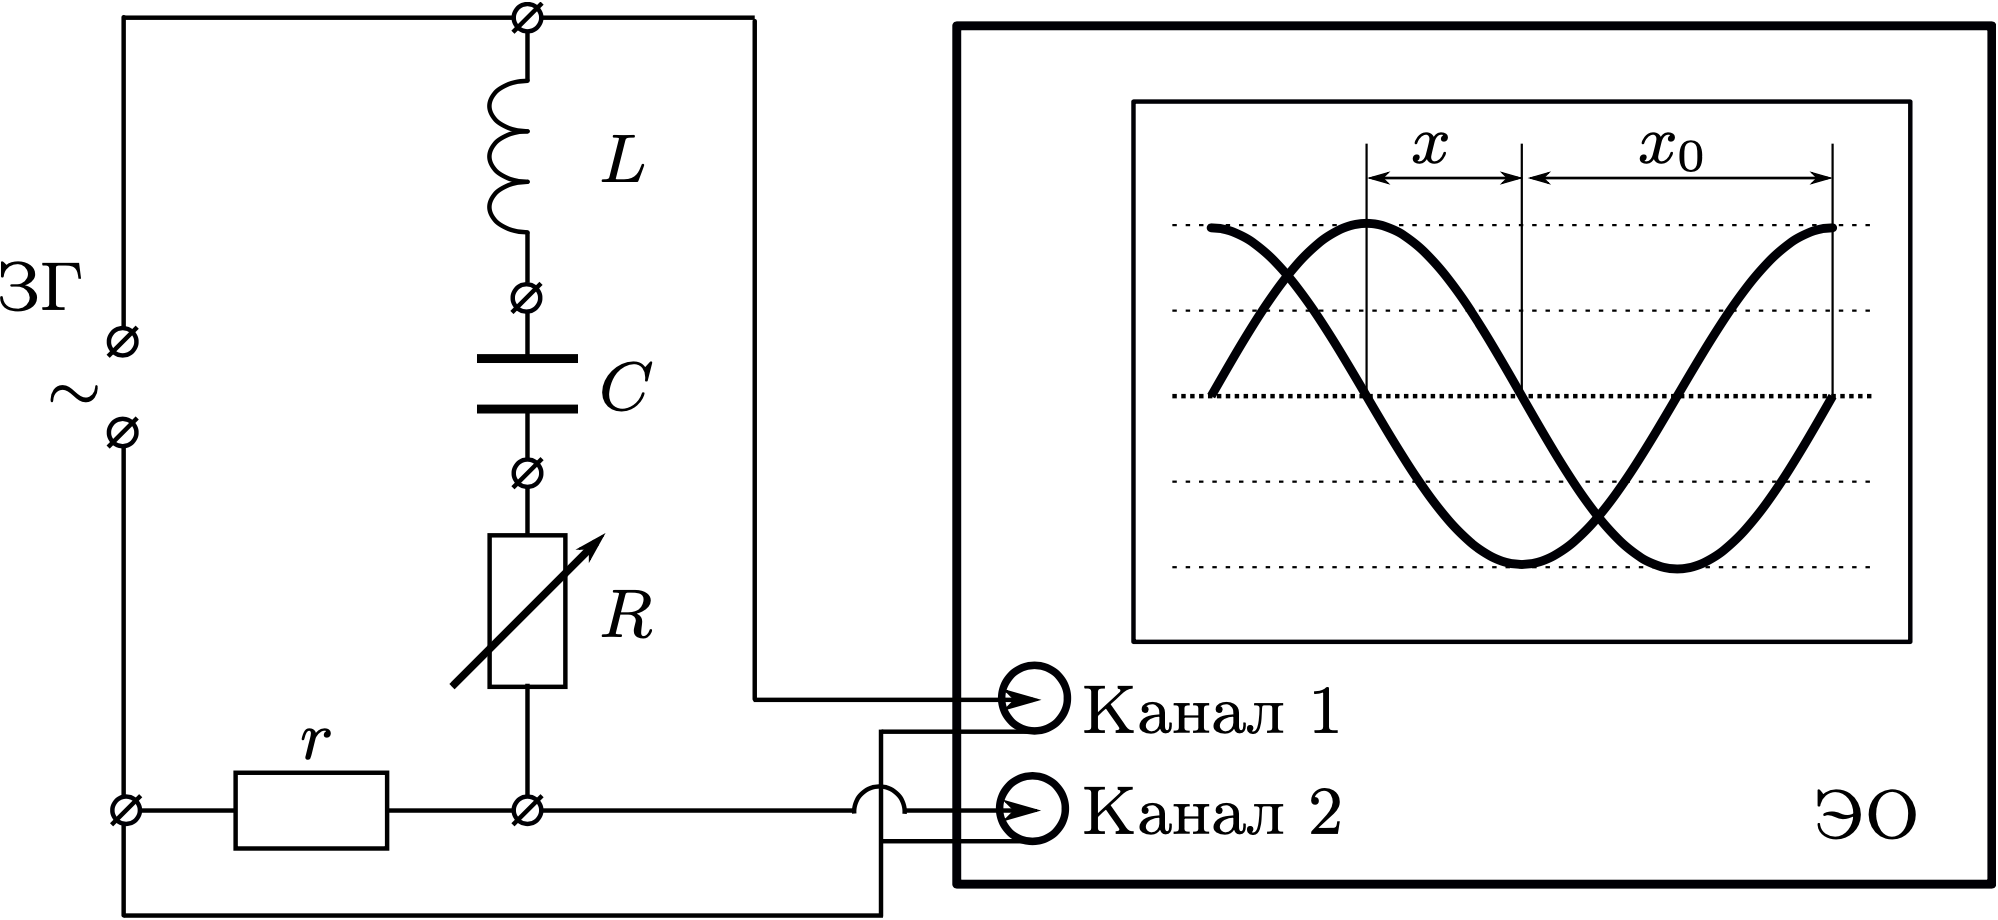
\includegraphics[width=0.5\linewidth]{images/picture1.png}
        \caption{Схема установки для исследования сдвига фаз между током и напряжением}
        \label{pic1}
    \end{figure}
    
    Сигнал, пропорциональный току, снимается c сопротивления $r$, пропорциональный напряжению, — с генератора. Оба сигнала подаются на осциллограф (ЭО), имеющий два канала вертикального отклонения. Измерение разности фаз можно проводить одним из двух описанных выше способов.
    
    На практике часто используются устройства, называемые \textit{фазовращателями}, которые позволяют изменять фазу напряжения в широких пределах (0 < $\psi$ < $\pi$). Схема фазовращателя, применяемого в данной работе, изображена на рис. \ref{pic2}. Она содержит два одинаковых резистора $R_1$, смонтированных на отдельной плате, магазин сопротивлений $R$ и магазин ёмкостей $C$.
    
    Найдём, как зависит сдвиг фаз между входным напряжением $U_{вх} = U_0 \cdot \mathrm{cos}(\omega t)$ (точки 1 и 2 на рис. \ref{pic2}) и выходным напряжением $U_{вых}$ (точки 3 и 4) от соотношения между импедансами сопротивления $R$ и ёмкости $C$. Для соответствующих комплексных амплитуд имеет место соотношение:
    \begin{equation}
        U_{вых} = \frac{U_{вх}}{2} \frac{R + \frac{i}{\omega C}}{R - \frac{i}{\omega C}}.
        \label{eq2}
    \end{equation}
    Числитель и знаменатель \eqref{eq2} — комплексно-сопряжённые величины, модули которых одинаковы. Поэтому амплитуда выходного напряжения не зависит от $R$, и всегда равна $U_0 / 2$. Сдвиг фаз между выходным и входным напряжениями равен
    \begin{equation}
        \psi = \mathrm{arg} \left( \frac{U_{вых}}{U_{вх}} \right) = 2 \cdot \mathrm{arctg} \left( \frac{1}{\omega R C} \right).
        \label{eq3}
    \end{equation}
    Он может меняться от $\psi = \pi$ при $R \rightarrow 0$ до $\psi = 0$ при $R \rightarrow \infty$.
    
    \begin{figure}[ht]
        \centering
        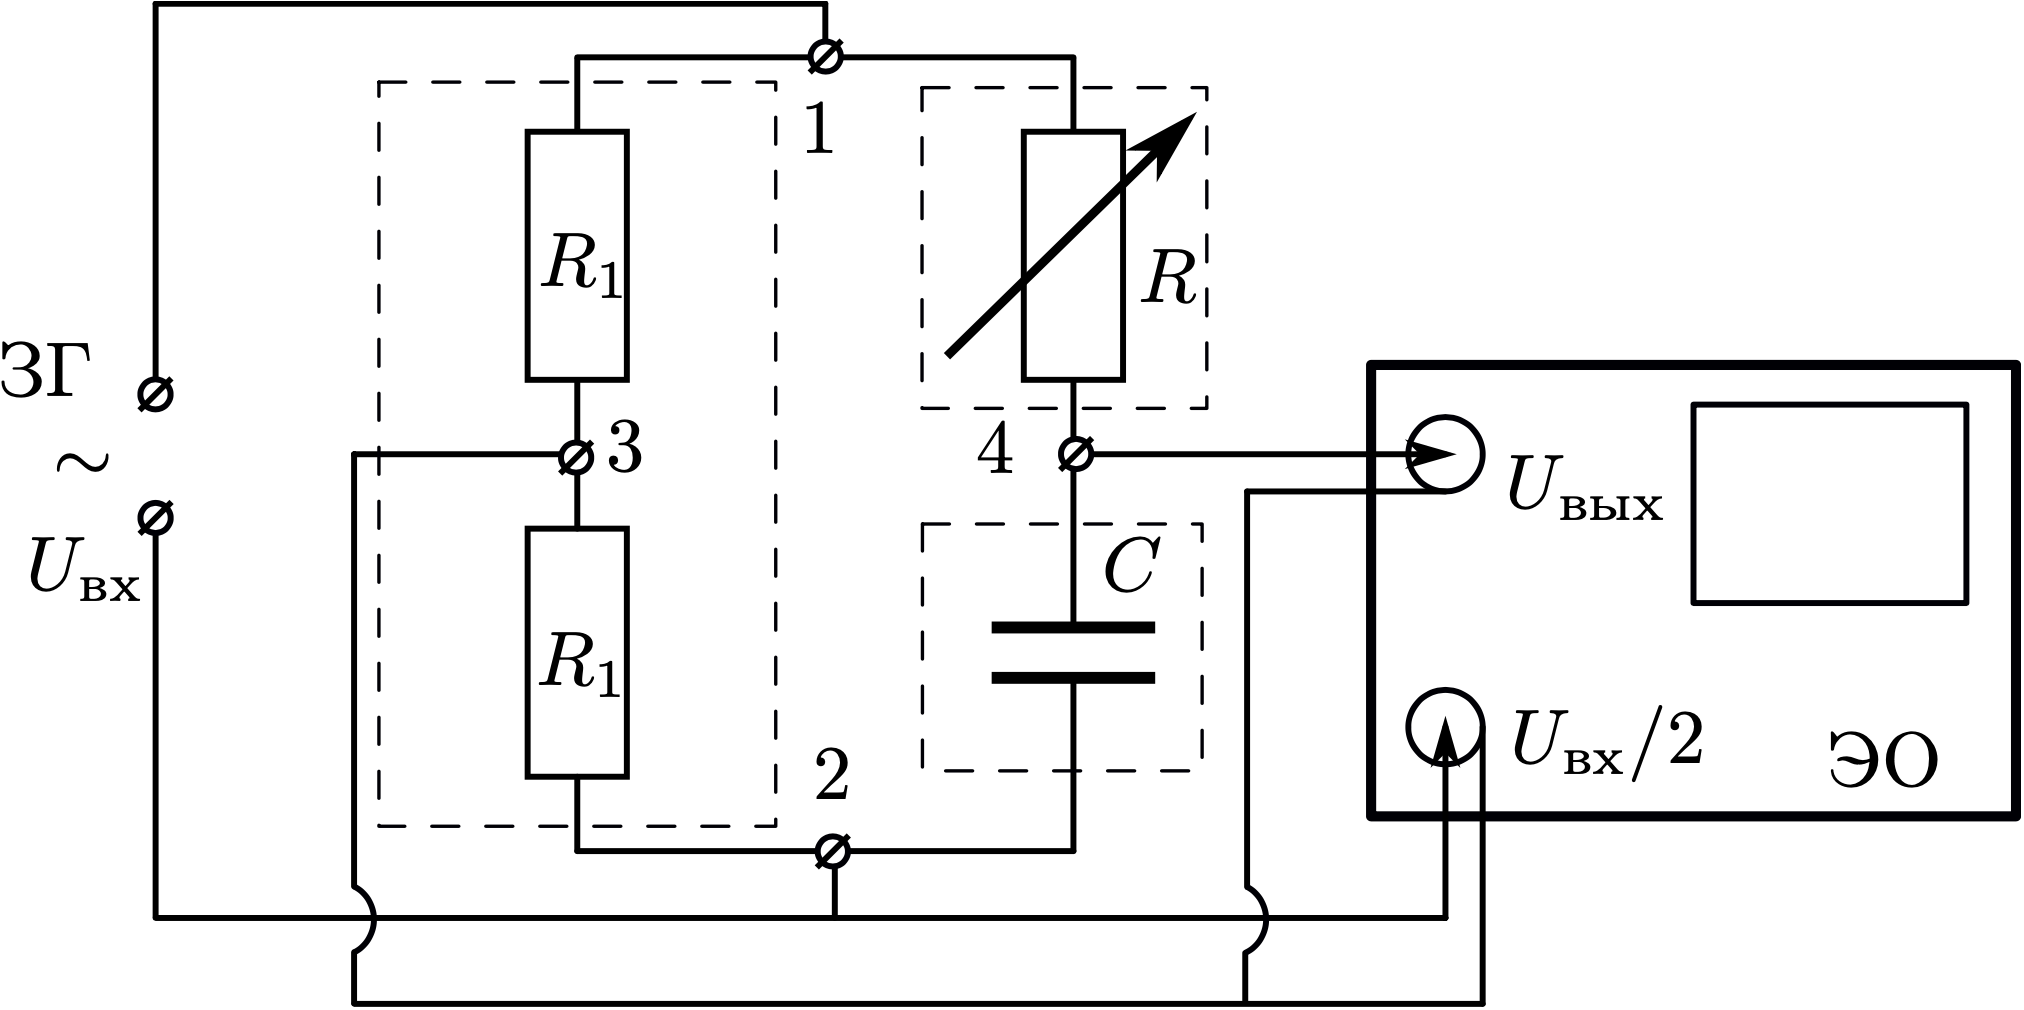
\includegraphics[width=0.5\linewidth]{images/picture2.png}
        \caption{Схема установки для исследования фазовращателя}
        \label{pic2}
    \end{figure}
    
    \newpage
    
    \begin{flushleft}
        {\Large {\bf Ход работы/Обработка результатов эксперимента}}
    \end{flushleft}
    
    {\bf 1. RC-цепь.} Запишем параметры установки: ёмкость конденсатора $C = 0,5 \text{ мкФ}$, сопротивление $r = 12,4 \text{ Ом}$, частота источника $\nu = 1000 \text{ Гц}$. Модуль реактивного сопротивления равен: $X_1 = \frac{1}{\omega C} = 318,3 \text{ Ом}$. Измерим зависимость сдвига фаз от сопротивления $R$ в диапазоне от $300 \text{ Ом}$ до $3200 \text{ Ом}$. Для этого будем измерять сдвиг $x$ одной синусоиды относительно другой в делениях экрана осцилографа и половину периода одной из синусоид $x_0$. Для повышения точности будем увеличивать синусоиду, дабы лучше разрешить сдвиг. Полученные результаты занесём в табл. \ref{table1}.
    
    \begin{table}[ht]
        \centering
        \begin{tabular}{|c|c|c|c|c|c|}
            \hline
            $R$, $\text{Ом}$ & $x_0$, $\text{дел}$ & $x$, $\text{дел}$ & $\Delta x$, $\text{дел}$ & $\psi$, $\text{рад}$ & $\Delta \psi$, $\text{рад}$ \\
            \hline
            318,31 & 5,0 & 1,2 & 0,10 & 0,75 & 0,06 \\
            \hline
            636,62 & 5,0 & 0,8 & 0,10 & 0,55 & 0,07 \\
            \hline
            1273,24 & 5,0 & 0,4 & 0,10 & 0,27 & 0,07 \\
            \hline
            1591,55 & 5,0 & 0,3 & 0,10 & 0,20 & 0,07 \\
            \hline
            1909,86 & 10,2 & 0,6 & 0,05 & 0,18 & 0,02 \\
            \hline
            2546,48 & 10,2 & 0,4 & 0,05 & 0,12 & 0,02 \\
            \hline
            2864,79 & 10,2 & 0,4 & 0,05 & 0,12 & 0,02 \\
            \hline
            3183,10 & 10,2 & 0,3 & 0,05 & 0,09 & 0,02 \\
            \hline
        \end{tabular}
        \caption{Зависимость сдвига фаз от сопротивления в RC-цепи}
        \label{table1}
    \end{table}
    
    Согласно теории мы должны получить зависимость:
    \begin{equation}
        \mathrm{tan}(\psi) = \frac{1}{\omega C R_{\Sigma}}.
    \end{equation}
    
    \begin{table}[ht]
        \centering
        \begin{tabular}{|c|c|c|c|c|c|c|c|c|}
            \hline
            $\mathrm{tan}(\psi)$ & 0,94 & 0,61 & 0,27 & 0,21 & 0,19 & 0,12 & 0,12 & 0,09 \\
            \hline
            $\Delta \mathrm{tan}(\psi)$ & 0,06 & 0,07 & 0,07 & 0,07 & 0,02 & 0,02 & 0,02 & 0,02 \\
            \hline
            $1/\omega C R_{\Sigma}$ & 0,96 & 0,49 & 0,25 & 0,20 & 0,17 & 0,12 & 0,11 & 0,10 \\
            \hline
        \end{tabular}
        \caption{Данные для построения графика $\mathrm{tan}(\psi) = f(1/\omega C R_{\Sigma})$}
    \end{table}
    
    \begin{figure}[ht]
        \centering
        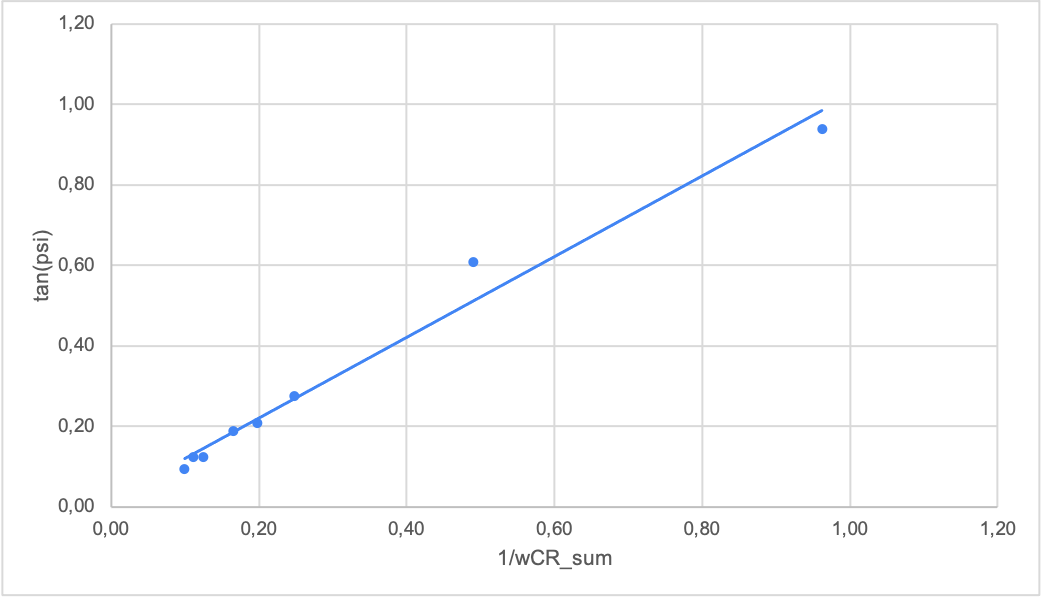
\includegraphics[width=0.79\linewidth]{images/RC-graph.png}
        \caption{График зависимости $\mathrm{tan}(\psi) = f(1/\omega C R_{\Sigma}),$ ($k = 1,00 \pm 0,05$)}
    \end{figure}
    
    \newpage
    
    {\bf 2. RL-цепь.} Аналогично RC-цепи проведём замеры и занесём все данные в табл. \ref{table2}. Реактивное сопротивление: $X_2 = \omega L = 314,2 \text{ Ом}$.
    
    \begin{table}[ht]
        \centering
        \begin{tabular}{|c|c|c|c|c|c|}
            \hline
            $R$, $\text{Ом}$ & $x_0$, $\text{дел}$ & $x$, $\text{дел}$ & $\Delta x$, $\text{дел}$ & $\psi$, $\text{рад}$ & $\Delta \psi$, $\text{рад}$ \\
            \hline
            314,16 & 8,2 & 3,5 & 0,10 & 1,34 & 0,04 \\
            \hline
            628,32 & 8,2 & 3,3 & 0,10 & 1,26 & 0,04 \\
            \hline
            1256,64 & 8,2 & 2,7 & 0,10 & 1,03 & 0,04 \\
            \hline
            1570,80 & 8,2 & 2,5 & 0,10 & 0,96 & 0,04 \\
            \hline
            1884,95 & 8,2 & 2,3 & 0,10 & 0,88 & 0,04 \\
            \hline
            2513,27 & 8,2 & 2,0 & 0,10 & 0,77 & 0,04 \\
            \hline
            2827,43 & 8,2 & 1,8 & 0,10 & 0,69 & 0,04 \\
            \hline
            3141,59 & 8,2 & 1,6 & 0,10 & 0,61 & 0,04 \\
            \hline
        \end{tabular}
        \caption{Зависимость сдвига фаз от сопротивления RL-цепи}
        \label{table2}
    \end{table}
    
    Согласно теории мы должны получить зависимость:
    \begin{equation}
        \mathrm{tan}(\psi) = \frac{\omega L}{R_{\Sigma}}.
    \end{equation}
    
    \begin{table}[ht]
        \centering
        \begin{tabular}{|c|c|c|c|c|c|c|c|c|}
            \hline
            $\mathrm{tan}(\psi)$ & 4,27 & 3,16 & 1,68 & 1,42 & 1,21 & 0,96 & 0,82 & 0,70 \\
            \hline
            $\Delta \mathrm{tan}(\psi)$ & 0,04 & 0,04 & 0,04 & 0,04 & 0,04 & 0,04 & 0,04 & 0,04 \\
            \hline
            $\omega L / R_{\Sigma}$ & 0,96 & 0,49 & 0,25 & 0,20 & 0,17 & 0,12 & 0,11 & 0,10 \\
            \hline
        \end{tabular}
        \caption{Данные для построения графика $\mathrm{tan}(\psi) = f(\omega L / R_{\Sigma})$}
    \end{table}
    
    \begin{figure}[ht]
        \centering
        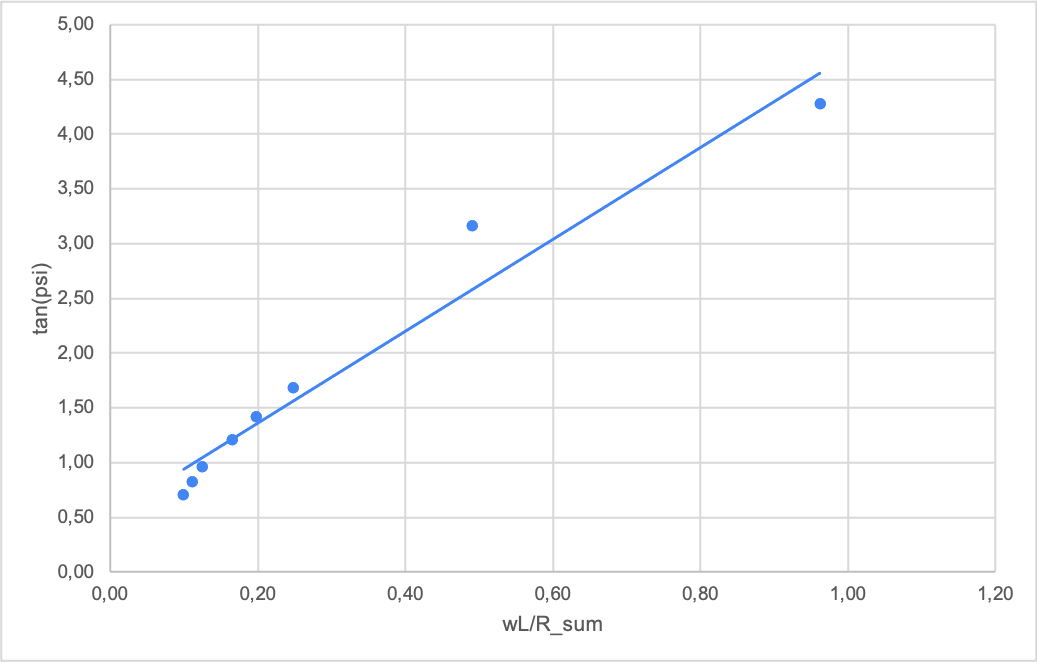
\includegraphics[width=0.84\linewidth]{images/RL-graph.png}
        \caption{График зависимости $\mathrm{tan}(\psi) = f(\omega L / R_{\Sigma})$, ($k = 4,20 \pm 0,33$)}
    \end{figure}
    
    \newpage
    
    {\bf 3. RLC-цепь.} Для RLC-цепи рассчитаем частоту резонанса ($C = 0,5 \text{ мкФ}$, $r = 12,4 \text{ Ом}$, $L = 50 \text{ мГн}$):
    \begin{equation}
        \nu_0 = \frac{1}{2 \pi \sqrt{L C}} = 1007 \text{ Гц}.
    \end{equation}
    
    \begin{table}[ht]
        \centering
        \begin{tabular}{|c|c|c|c|c|c|c|c|}
            \hline
            \multicolumn{4}{|c|}{$R = 0 \text{ Ом}$} & \multicolumn{4}{c|}{$R = 100 \text{ Ом}$} \\
            \hline
            $\nu$, $\text{Гц}$ & $x_0$ & $x$ & $|\psi|$ & $\nu$, $\text{Гц}$ & $x_0$ & $x$ & $|\psi|$ \\
            \hline
            870 & 2,9 & 1,0 & 1,08 & 800 & 3,1 & 0,8 & 0,81 \\
            \hline
            900 & 2,8 & 0,9 & 1,01 & 850 & 3,0 & 0,6 & 0,63 \\
            \hline
            930 & 2,7 & 0,6 & 0,70 & 900 & 2,8 & 0,4 & 0,45 \\
            \hline
            960 & 2,6 & 0,4 & 0,48 & 950 & 2,5 & 0,2 & 0,25 \\
            \hline
            1000 & 2,5 & 0,05 & 0,06 & 1000 & 2,5 & 0 & 0 \\
            \hline
            1030 & 2,4 & 0,4 & 0,52 & 1050 & 2,4 & 0,2 & 0,26 \\
            \hline
            1060 & 2,4 & 0,6 & 0,79 & 1100 & 2,4 & 0,4 & 0,52 \\
            \hline
            1090 & 2,3 & 0,7 & 0,96 & 1150 & 2,2 & 0,6 & 0,86 \\
            \hline
        \end{tabular}
        \caption{Сдвиг фаз в RLC-цепи}
    \end{table}
    
    \begin{table}[ht]
        \centering
        \begin{tabular}{|c|c|c|c|c|c|c|c|c|}
            \hline
            \multicolumn{9}{|c|}{$R = 0 \text{ Ом}$} \\
            \hline
            $|\psi| / \pi$ & 0,34 & 0,32 & 0,22 & 0,15 & 0,02 & 0,17 & 0,25 & 0,30 \\
            \hline
            $\nu / \nu_0$ & 0,86 & 0,89 & 0,92 & 0,95 & 0,99 & 1,02 & 1,05 & 1,08 \\
            \hline
            \multicolumn{9}{|c|}{$R = 100 \text{ Ом}$} \\
            \hline
            $|\psi| / \pi$ & 0,26 & 0,20 & 0,14 & 0,08 & 0,00 & 0,08 & 0,17 & 0,27 \\
            \hline
            $\nu / \nu_0$ & 0,79 & 0,84 & 0,89 & 0,94 & 0,99 & 1,04 & 1,09 & 1,14 \\
            \hline
        \end{tabular}
        \caption{Данные для построения графика $|\psi| / \pi = f(\nu / \nu_0)$}
    \end{table}
    
    Результаты таблицы отразим в графике на рис. \ref{pic3}. Синими точками показано изменение сдвига фаз при $R = 0 \text{ Ом}$, красными – при $R = 100 \text{ Ом}$.
    
    Рассчитаем добротность цепи экспериментально по формуле:
    \begin{equation}
        Q = \frac{\nu_0}{2 \Delta \nu},
    \end{equation}
    получим
    \begin{equation}
        Q_0 = 6,9 \pm 1,8 \hspace{1.5cm} Q_{100} = 3,0 \pm 0,4.
    \end{equation}
    Рассчитаем добротность цепи теоретически по формуле:
    \begin{equation}
        Q = \frac{1}{R} \sqrt{\frac{L}{C}},
    \end{equation}
    получим
    \begin{equation}
        Q_0 = 6,8 \hspace{1.5cm} Q_{100} = 2,2.
    \end{equation}
    
    \begin{figure}[ht]
        \centering
        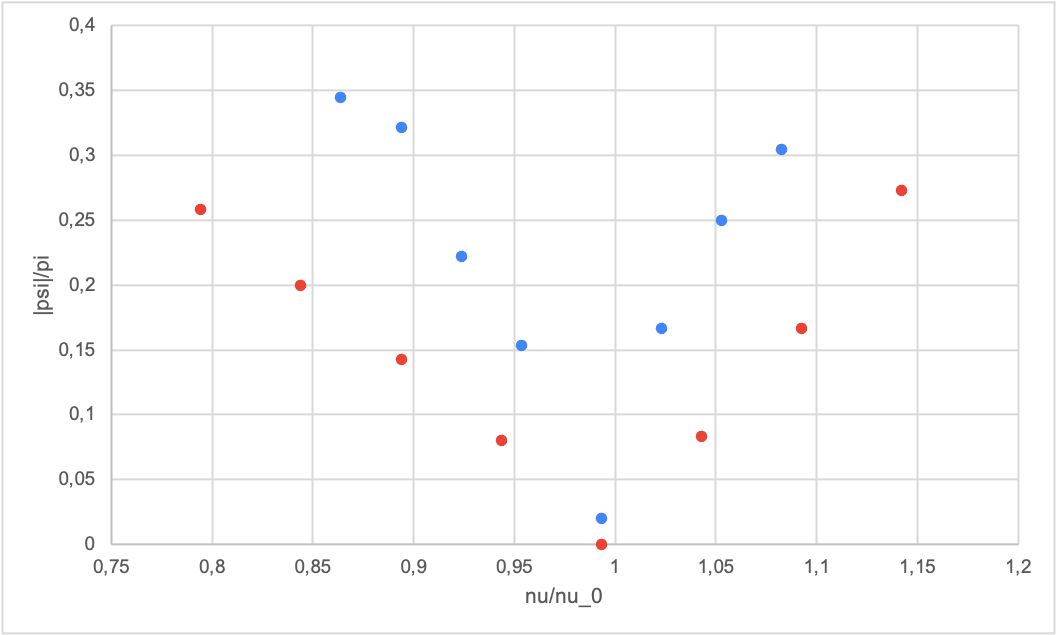
\includegraphics[width=0.9\linewidth]{images/RLC-graph.png}
        \caption{График зависимости $|\psi| / \pi = f(\nu / \nu_0)$}
        \label{pic3}
    \end{figure}
    
    \newpage
    
    {\bf Фазовращатель.} Нарисуем векторную диаграмму для случая $\psi = \pi / 2$:
    
    \begin{figure}[ht]
        \centering
        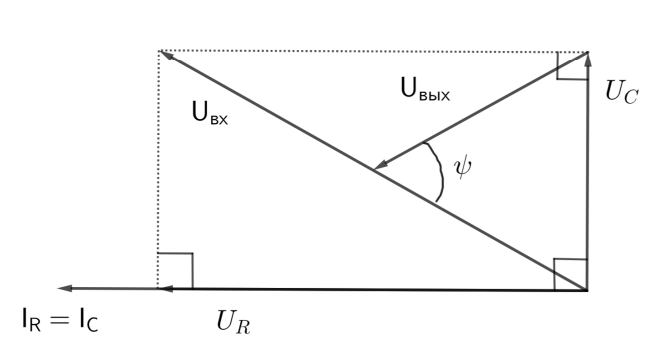
\includegraphics{images/phase.png}
        \caption{Векторная диаграмма для $\psi = \pi / 2$}
    \end{figure}
    
    По расчётам получим $R = 318,5 \text{ Ом}$. На практике же получили значение $R = 330 \pm 10 \text{ Ом}$. Погрешность при практическом измерении оценена как шаг дискретезации (поворот какой-либо из ручек магазина), при котором отсутствуют заметные глазу изменения на осциллографе.
    
    \begin{flushleft}
        {\Large {\bf Вывод}}
    \end{flushleft}
    
    В ходе данной лабораторной работы была проверена теоретическая зависимость сдвига фаз от параметров системы, экспериментально была рассчитана добротность системы в RLC-цепи и сравнена с теоретическим значением. Результат, полученный при изучении RL-цепи, не совпал с теоретическими прогнозами. Скорее всего, данное несовпадение случилось в следствие неисправности оборудования (т.к. во время проведения лабораторной работы экспериментаторы столкнулись с рядом трудностей в работе приборов), но не исключается и факт ошибки экспериментаторов.
    
\end{document}